\documentclass[12pt, twoside]{article}
\usepackage[letterpaper, margin=1in, headsep=0.5in]{geometry}
\usepackage[english]{babel}
\usepackage[utf8]{inputenc}
\usepackage{amsmath}
\usepackage{amsfonts}
\usepackage{amssymb}
\usepackage{tikz}
\usepackage{yhmath}
%\usetikzlibrary{quotes, angles}

\usepackage{graphicx}
\usepackage{enumitem}
\usepackage{multicol}

\usepackage{fancyhdr}
\pagestyle{fancy}
\fancyhf{}
\renewcommand{\headrulewidth}{0pt} % disable the underline of the header

\fancyhead[RE]{\thepage}
\fancyhead[RO]{\thepage \\ Name: \hspace{3cm}}
\fancyhead[L]{BECA / Dr. Huson / 10th Grade Geometry\\* 16 May 2019}

\begin{document}
\subsubsection*{11.5 Do Now: Density \& compound shapes}
 \begin{enumerate}
  \item A lamp fixture is in the shape of a triangular pyramid. It is 7.2 inches tall and the area of its base is 11.5 in$^2$. Find the volume of the fixture to the \emph{nearest cubic inch}. \vspace{3cm}

  \item A marble statue has a volume of 1135 in$^3$. Find its weight, to the \emph{nearest tenth of a pound}. (assume the density of marble is 1.57 \emph{ounces} per cubic inch) \vspace{3cm}

  \item The area of the Bronx, NY is 42.47 square miles. Its population density is approximately 34,600 people per square mile. Estimate the population of the Bronx. \vspace{3cm}

  \item The volume of a cone is found to be 414.7 using the following formula:
    \[V=\frac{1}{3} \pi r^2 \times 11=414.7\]
    What does the value $11$ in the formula represent? Solve for the radius. \vspace{7cm}

\newpage
  \item BECA middle schoolers draw a basketball key on the asphalt in chalk. It is rectangular with one end round. It is 6 feet wide and overall it is 11 feet long, as shown. Find the area of the chalked basketball key to the \emph{nearest square foot}.\\[1.5cm]
    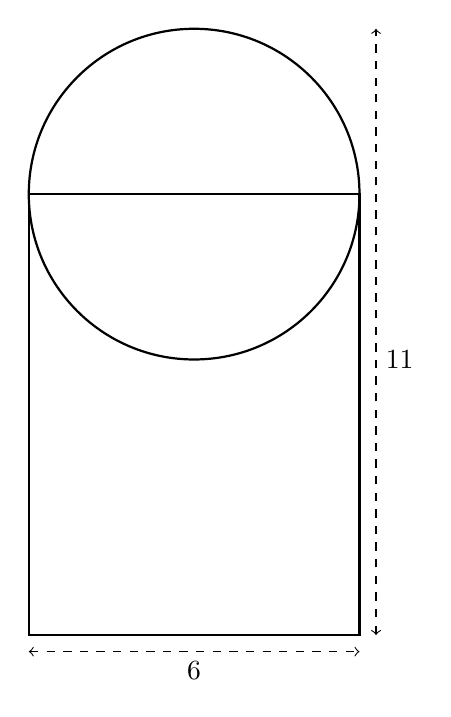
\begin{tikzpicture}[scale=0.7]
      \draw [thick]
      (0,0)--(0,8)--(6,8)--(6,0)--cycle;
      \draw [thick] (3,8) circle[radius=3];
      \draw [dashed,<->] (6.3,0)--(6.3,11);
      \draw [dashed,<->] (0,-0.3)--(6,-0.3);
      %\draw (0,8)++(0,-0.8)--++(0.8,0)--+(0,0.8);
      \node at (3,-0.3)[below]{$6$};
      \node at (6.3,5)[right]{$11$};
      %\node at (6.25,7)[right]{$2$};
    \end{tikzpicture}

  \item A wooden plank is laid on a brick platform. There are three steps leading to the platform, each 1 foot tall. The length of the plank is 16 feet. What is the angle of elevation, $x$, that the plank makes with the ground, to the \emph{nearest degree}.\\[1.cm]
        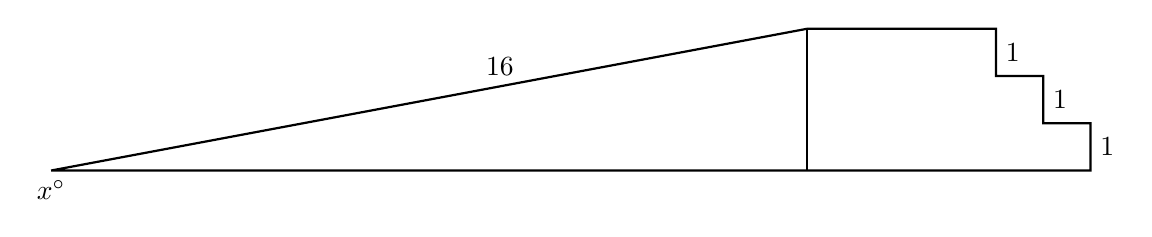
\begin{tikzpicture}[scale=0.6]
          \draw [thick] (-6,0)--(10,3)--(14,3)--(14,2)--(15,2)--(15,1)--(16,1)--(16,0)--cycle;
          \draw [thick] (10,0)--(10,3);
          %\draw (10,16)++(0,-0.8)--++(0.8,0)--+(0,0.8);
          \node at (16,0.5)[right]{$1$};
          \node at (15,1.5)[right]{$1$};
          \node at (14,2.5)[right]{$1$};
          \node at (-6,0)[below]{$x^\circ$};
          \node at (3.5, 1.8)[above]{$16$};
          %\node at (14, 4)[above]{\emph{Not to Scale}};
        \end{tikzpicture} \vspace{5cm}

  \end{enumerate}
  \newpage
  \setcounter{page}{1}
\subsubsection*{11.5 Pop Quiz: Density \& compound shapes}
 \begin{enumerate}

\item A candle has the shape of a cone. It is 8.5 inches tall and the diameter of its base is 4 inches. Find the volume of the candle to the \emph{nearest cubic inch}. \vspace{3cm}

\item A bronze trophy has a volume of 520 cm$^3$. Find its weight, to the \emph{nearest tenth of a kilogram}. (assume the density of bronze is $8.5 \ grams/ \mathrm{cm}^3$) \vspace{2.5cm}

\item The area of Manhattan, NY is 22.82 square miles. Its population density is approximately 73,000 people per square mile. Estimate the population of Manhattan. \vspace{2.5cm}

\item The volume of a pyramid with a square base is found to be 245 using the formula:
  \[V=\frac{1}{3} x^2 \times 15=245\]
  What does the value $15$ in the formula represent? Solve for the length of the side of the square base. \vspace{7cm}

\newpage
\item Mott Hall fourth graders draw a basketball key on the asphalt in chalk. It is rectangular with one end round. It is 4 feet wide and overall it is 7 feet long, as shown. Find the area of the chalked basketball key to the \emph{nearest square foot}.\\[1.5cm]
  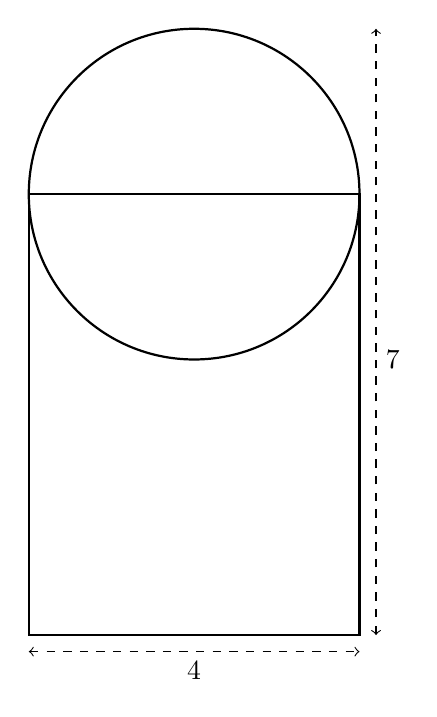
\begin{tikzpicture}[scale=0.7]
    \draw [thick]
    (0,0)--(0,8)--(6,8)--(6,0)--cycle;
    \draw [thick] (3,8) circle[radius=3];
    \draw [dashed,<->] (6.3,0)--(6.3,11);
    \draw [dashed,<->] (0,-0.3)--(6,-0.3);
    %\draw (0,8)++(0,-0.8)--++(0.8,0)--+(0,0.8);
    \node at (3,-0.3)[below]{$4$};
    \node at (6.3,5)[right]{$7$};
    %\node at (6.25,7)[right]{$2$};
  \end{tikzpicture}

\item A wooden plank is laid on a brick platform. There are two steps leading to the platform, each 1 foot tall. The length of the plank is 10 feet. What is the angle of elevation, $x$, that the plank makes with the ground, to the \emph{nearest degree}.\\[1.cm]
      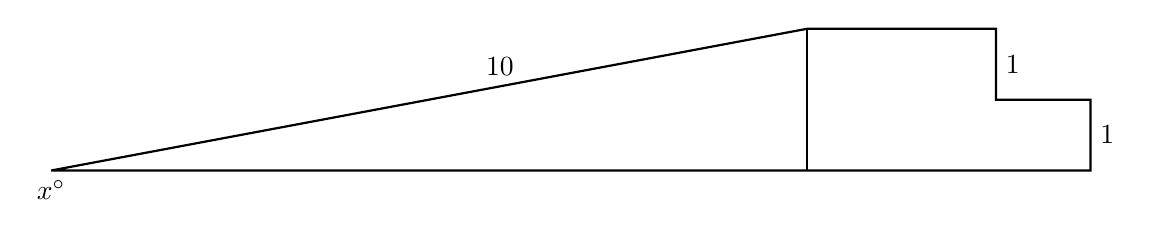
\begin{tikzpicture}[scale=0.6]
        \draw [thick] (-6,0)--(10,3)--(14,3)--(14,1.5)--(16,1.5)--(16,0)--cycle;
        \draw [thick] (10,0)--(10,3);
        %\draw (10,16)++(0,-0.8)--++(0.8,0)--+(0,0.8);
        \node at (16,0.75)[right]{$1$};
        \node at (14,2.25)[right]{$1$};
        \node at (-6,0)[below]{$x^\circ$};
        \node at (3.5, 1.8)[above]{$10$};
        %\node at (14, 4)[above]{\emph{Not to Scale}};
      \end{tikzpicture} \vspace{5cm}



  \end{enumerate}
  \newpage
  \setcounter{page}{1}
\subsubsection*{11.5 Homework: Using slope and distance formulas}
 \begin{enumerate}


   \item Given right $\triangle EFG$ with $m\angle G=90^\circ$. If $FG=8$ and $EG=6$, find $EF$.\\
       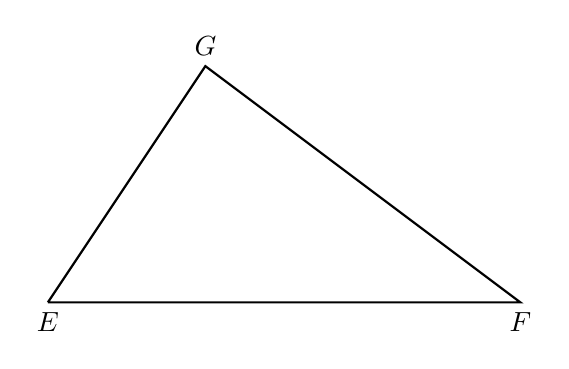
\begin{tikzpicture}%[scale=0.7]
         \draw [thick] (2,0)node[below]{$E$}--
           (8,0)node[below]{$F$}--
           (4,3)node[above]{$G$} --(2,0);
       \end{tikzpicture} \vspace{1cm}

    \item In the diagram below, $\triangle ABC$ has vertices with coordinates $A(0,3)$, $B(6,1)$ and $C(4,5)$.
      \begin{center} %4 quadrant regents grid
        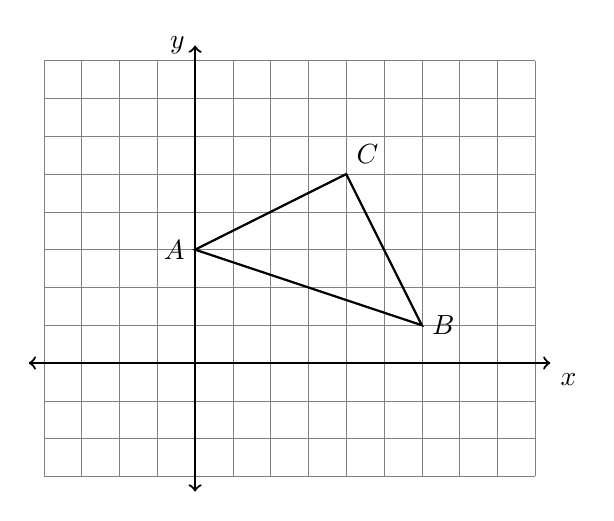
\begin{tikzpicture}[scale=.48]
          \draw [help lines] (-4,-3) grid (9,8);
          \draw [thick, <->] (-4.4,0) -- (9.4,0) node [below right] {$x$};
          \draw [thick, <->] (0,-3.4)--(0,8.4) node [left] {$y$};
          \draw [thick]
            (0,3)node[left]{$A$}--
            (6,1) node[right]{$B$}--
            (4,5) node[above right]{$C$}--cycle;
          %\draw [fill] (-1,2) circle [radius=0.1] node[above left] {$A$};
          %draw [fill] (8, -4) circle [radius=0.1] node[below right] {$C$};
        \end{tikzpicture}
      \end{center}
      Find the length of each side of $\triangle ABC$, showing that it is isosceles and not equilateral.\\[0.5cm]
        \begin{tabular}{c|c|c}
          $AC=$ & $BC=$ & $AB=$ \\
          $\sqrt{(x_C-x_A)^2+(y_C-y_A)^2}$ & $\sqrt{(x_C-x_B)^2+(y_C-y_B)^2}$ & $ \sqrt{(x_B-x_A)^2+(y_B-y_A)^2}$ \\
          & & \\
          & & \\
        \end{tabular}

\newpage

\end{enumerate}
\end{document}
